% Appendix A

\chapter{Arquitectura de la red y Resultados obtenidos} % Main appendix title


\label{AppendA} % For referencing this appendix elsewhere, use \ref{AppendixA}
\section{Arquitecturas}
\subsection{RNN simple}
\begin{figure}[H]
	\begin{center}
		\begin{tikzpicture}[node distance=2cm]
		\node (i1) [startstop] {Input Layer};
		\node (i2) [startstop, below of=i1] {Recurrent Layer};
		
		\node (i3) [startstop, below of=i2] {Dense Layer};
		\node (i4) [startstop, below of=i3] {Output Layer};
		\draw [arrow] (i1) -- (i2) ;
		\draw [arrow] (i2) -- (i3);
		\draw [arrow] (i3) -- (i4);
		\end{tikzpicture}
	\end{center}
	\caption{Esquema de  RNN simple \\ Fuente:  \textit{Fuente Propia}}
\end{figure}


\subsection{LSTM simple}
\begin{figure}[H]
	\begin{center}
		\begin{tikzpicture}[node distance=2cm]
		\node (i1) [startstop] {Input Layer};
		\node (i2) [startstop, below of=i1] {LSTM Layer};
		
		\node (i3) [startstop, below of=i2] {Dense Layer};
		\node (i4) [startstop, below of=i3] {Output Layer};
		\draw [arrow] (i1) -- (i2) ;
		\draw [arrow] (i2) -- (i3);
		\draw [arrow] (i3) -- (i4);
		\end{tikzpicture}
	\end{center}
	\caption{Esquema de LSTM simple \\ Fuente:  \textit{Fuente Propia}}
\end{figure}


\subsection{LSTM con Dropout}
\begin{figure}[H]
	\begin{center}
		\begin{tikzpicture}[node distance=2cm]
		\node (i1) [startstop] {Input Layer};
		\node (i2) [startstop, below of=i1] {LSTM Layer};
		\node (i3) [startstop, below of=i2] {Dropout};
		\node (i4) [startstop, below of=i3] {Dense Layer};
		\node (i5) [startstop, below of=i4] {Output Layer};
		\draw [arrow] (i1) -- (i2) ;
		\draw [arrow] (i2) -- (i3);
		\draw [arrow] (i3) -- (i4);
		\draw [arrow] (i4) -- (i5);
		\end{tikzpicture}
	\end{center}
	\caption{Esquema de LSTM con dropout \\ Fuente:  \textit{Fuente Propia}}
\end{figure}

\section{Resultados de precisión de entrenamiento}

\begin{figure}[H]
\centering
	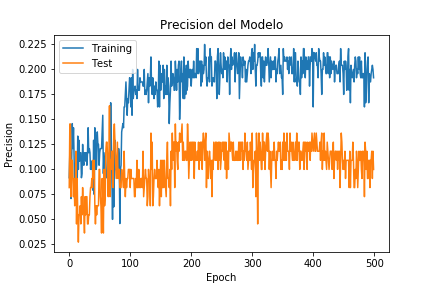
\includegraphics[width=0.8\textwidth]{Figures/RNNsimpleprec}
	\caption{Precisión de RNN para 500 epochs\\ Fuente: {\textit{Fuente Propia}}}
	\label{RNNSIMPLE}
\end{figure} 

\begin{figure}[H]
	\centering
	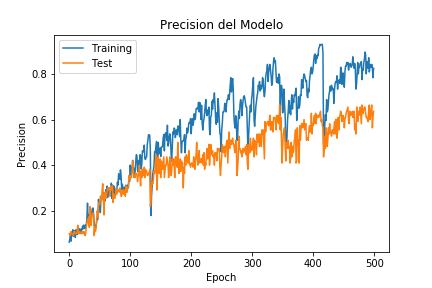
\includegraphics[width=0.8\textwidth]{Figures/LSTMsimpleprec}
	\caption{Precisión de LSTM simple para 500 epochs\\ Fuente: {\textit{Fuente Propia}}}
	\label{LSTMsimpel}
\end{figure} 

\begin{figure}[H]
	\centering
	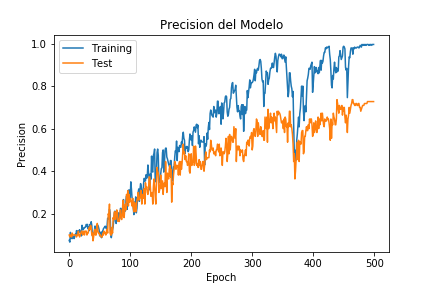
\includegraphics[width=0.8\textwidth]{Figures/LSTM_droprec05.png}
	\caption{Precisión de LSTM dropout 0.5 para 500 epochs\\ Fuente: {\textit{Fuente Propia}}}
	\label{LSTMdropout5}
\end{figure} 



\begin{figure}[H]
	\centering
	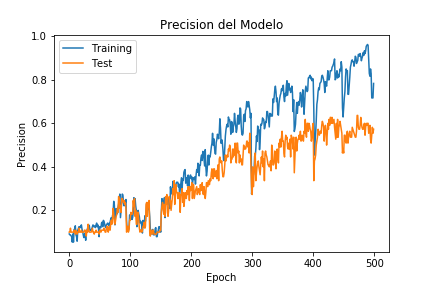
\includegraphics[width=0.8\textwidth]{Figures/lstm_drop08prec.png}
	\caption{Precisión de LSTM dropout 0.8 para 500 epochs\\ Fuente: {\textit{Fuente Propia}}}
	\label{LSTMdropout8}
\end{figure} 
\section{Resultados de función de perdida}

\begin{figure}[H]
	\centering
	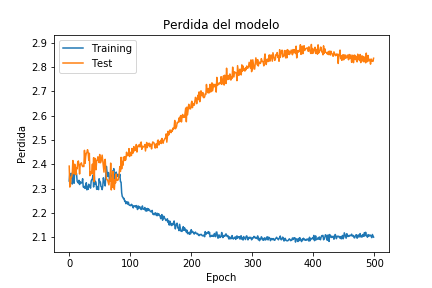
\includegraphics[width=0.8\textwidth]{Figures/RNNsimplecost}
	\caption{Perdida de RNN para 500 epochs\\ Fuente: {\textit{Fuente Propia}}}
	\label{RNNSIMPLEcost}
\end{figure} 


\begin{figure}[H]
	\centering
	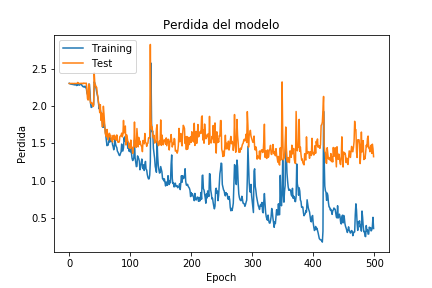
\includegraphics[width=0.8\textwidth]{Figures/LSTMsimplecost}
	\caption{Perdida de LSTM para 500 epochs\\ Fuente: {\textit{Fuente Propia}}}
	\label{LSTMsimplecost}
\end{figure} 

\begin{figure}[H]
	\centering
	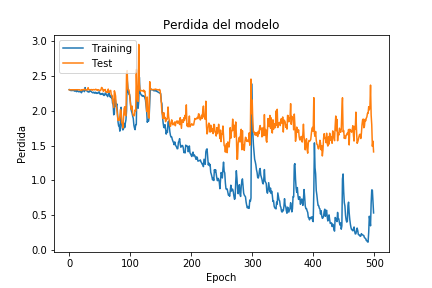
\includegraphics[width=0.8\textwidth]{Figures/lstm_drop08cost.png}
	\caption{Perdida de LSTM dropout 0.8 para 500 epochs\\ Fuente: {\textit{Fuente Propia}}}
	\label{LSTMdropout5cost}
\end{figure} 


\begin{figure}[H]
	\centering
	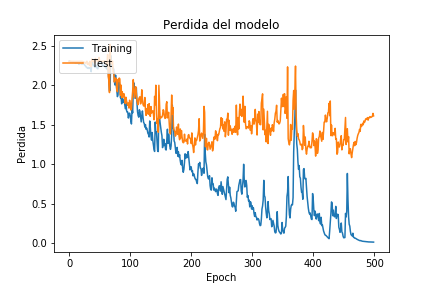
\includegraphics[width=0.8\textwidth]{Figures/LSTM_drocost05.png}
	\caption{Perdida de LSTM dropout 0.5 para 500 epochs\\ Fuente: {\textit{Fuente Propia}}}
	\label{LSTMdropout8cost}
\end{figure} 